\chapter{Discussion}
%

\section{Future Work}
\label{Future Work}
%%%%%%%%%%%%%%%%%%%%%%
%%%%%%%%%%%%%%%%%%%%%%
\section{Towards Automating the Image-to-Analysis Pipeline}
\label{Towards Automating the Image-to-Analysis Pipeline}
%%%%%%%%%%%%%%%%%%%%%%
%%%%%%%%%%%%%%%%%%%%%%
\subsection{Multiple Materials and Inhomogeneous Materials}
\label{Multiple Materials and Inhomogeneous Materials}
%%%%%%%%%%%%%%%%%%%%%%
%%%%%%%%%%%%%%%%%%%%%%
\subsection{Uncertainty Quantification, Verification, and Validation}
\label{Uncertainty Quantification, Verification, and Validation}
Material properties, boundary conditions
%%%%%%%%%%%%%%%%%%%%%%
%%%%%%%%%%%%%%%%%%%%%%
\subsection{High Performance Computing}
\label{High Performance Computing}
%%%%%%%%%%%%%%%%%%%%%%
%%%%%%%%%%%%%%%%%%%%%%
\section{Clinical Implications}
\label{Clinical Implications}
(haptics, Simpleware stuff)\\
Center for Cardiovascular simulation (Texas)
Heartflow, Inc., Charles Taylor

ASME V\&V10 and V\&V40

dental applications - 1) for implant placement and crown design, 2) for 3D printing, aesthetic try-in 

tolerance-aware voronoi-partitioning \\
multiple material interfaces (see paper) \\

Abaqus: ability to deal with initial over-closures? A strain-free adjustment perhaps? Like if you were to mesh the femur and the femoral cartilage separately, say, and there is a tiny bit of overlap between them..are you able to fix this without going back to the meshing software?  

\begin{figure}[tbh]
\centering
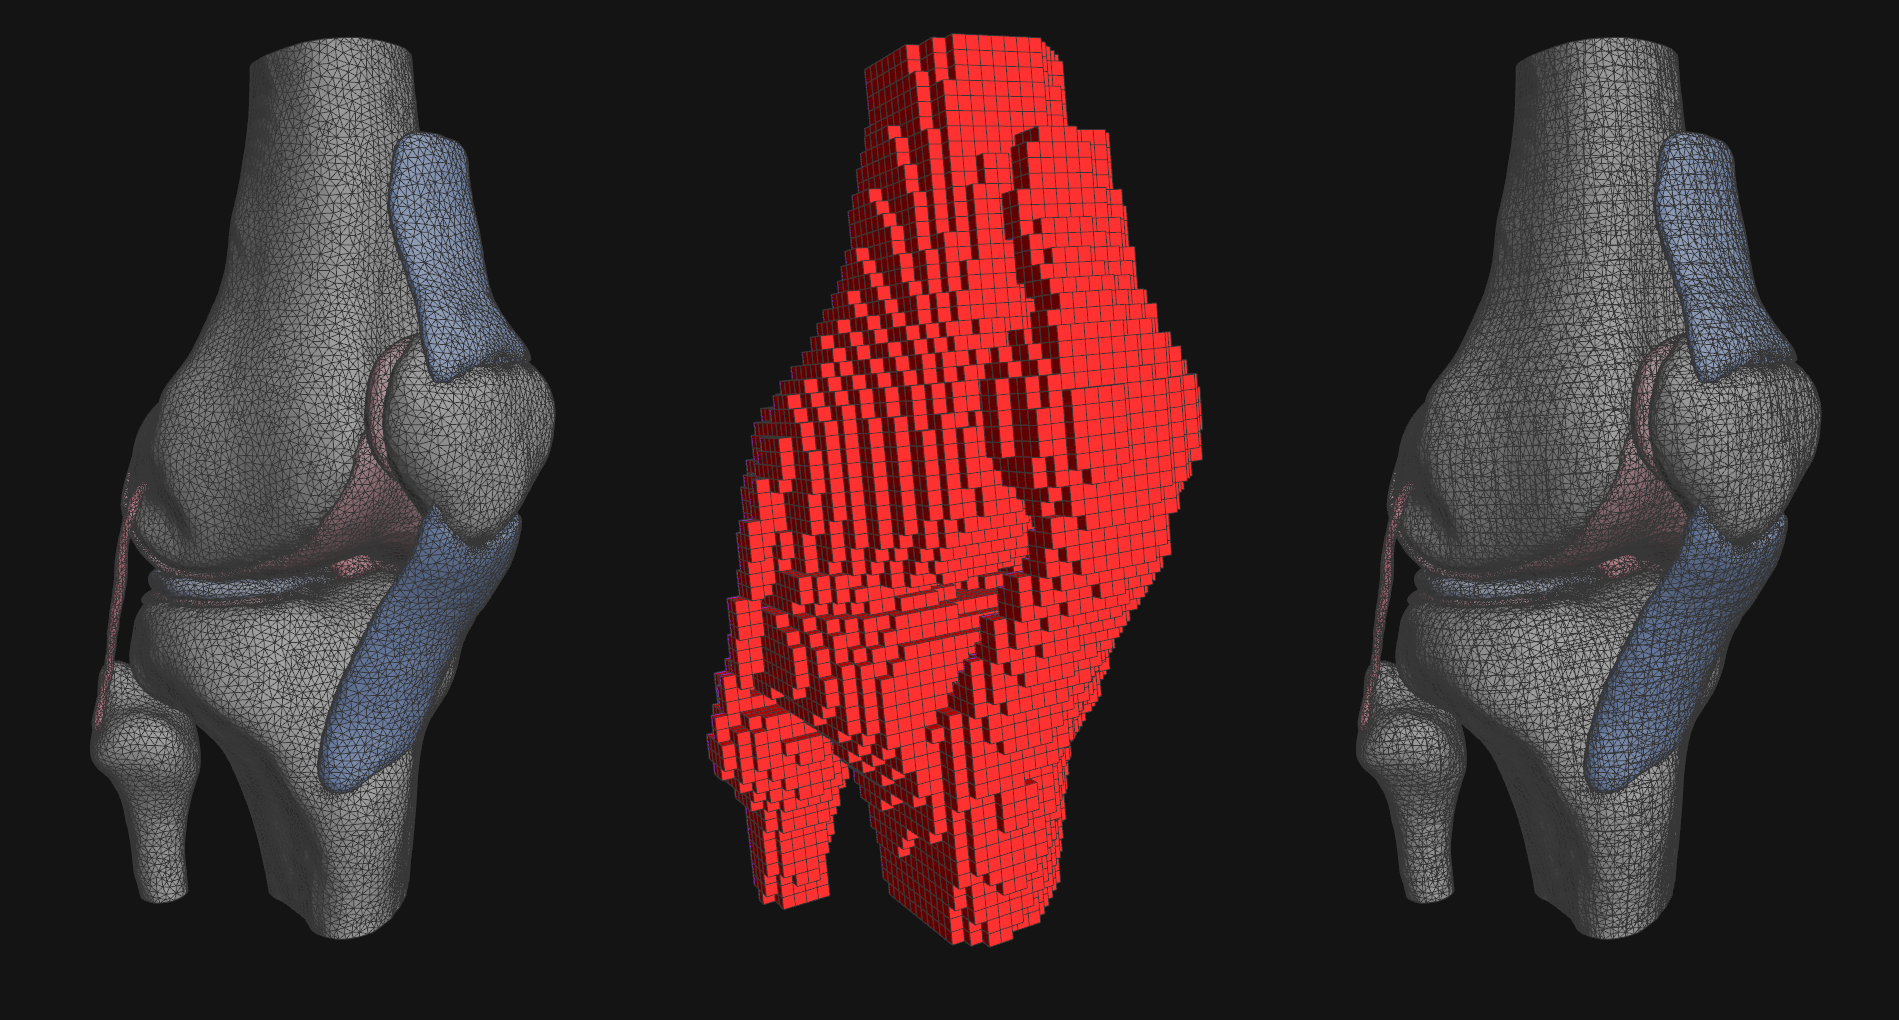
\includegraphics{media/sequence.png}
% where an .eps filename suffix will be assumed under latex,
% and a .pdf suffix will be assumed for pdflatex
\caption[sequence]{Sequence on knee.}
\label{fig.sequence}
\end{figure}

\begin{figure}[tbh]
\centering
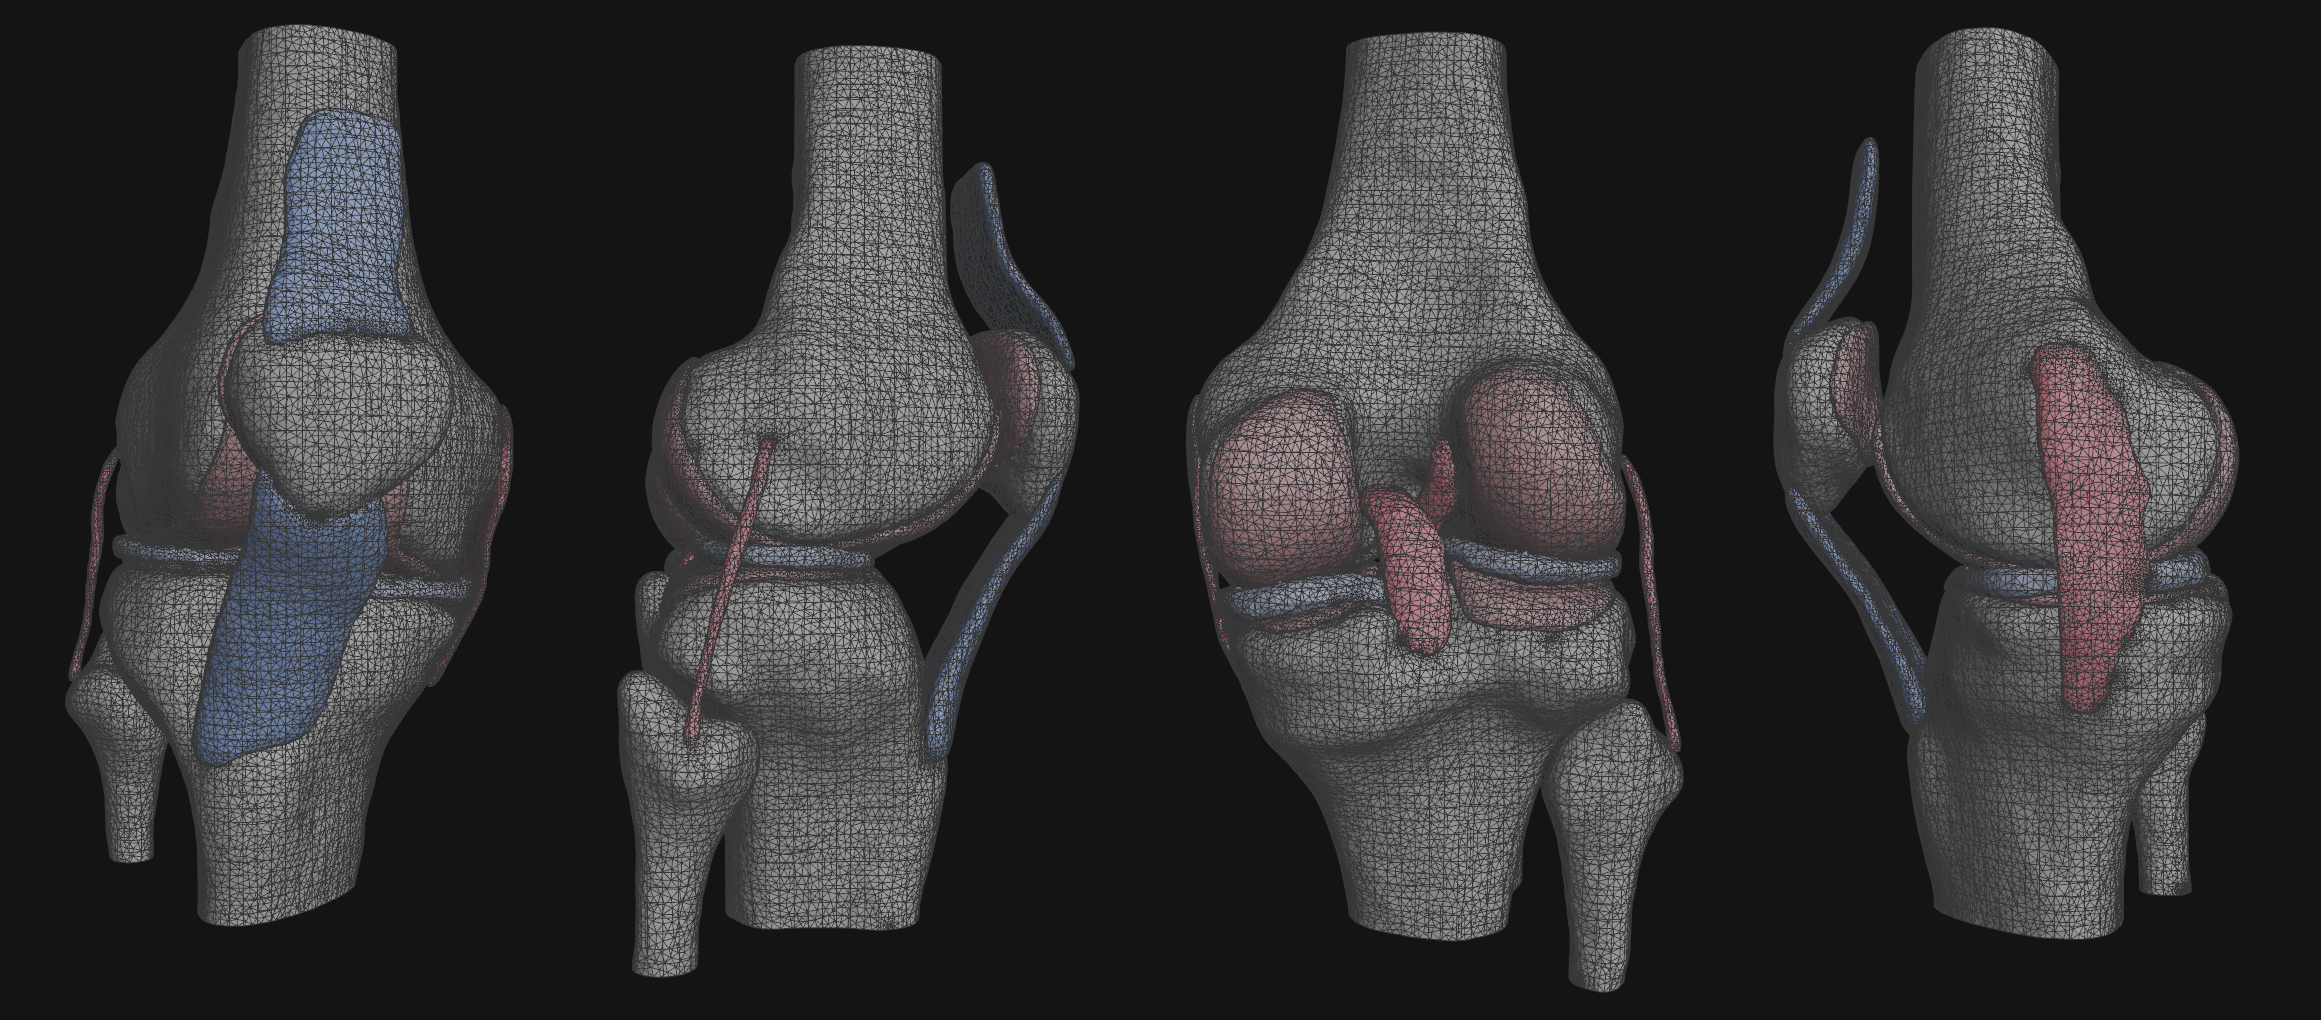
\includegraphics{media/fullmesh.png}
% where an .eps filename suffix will be assumed under latex,
% and a .pdf suffix will be assumed for pdflatex
\caption[polyhedral knee]{Polyhedral mesh of knee.}
\label{fig.sample_1}
\end{figure}